\documentclass[a0,portrait]{a0poster}

\usepackage{multicol}
\columnsep=100pt
\columnseprule=3pt

\usepackage[svgnames]{xcolor}
\usepackage{graphicx}
\usepackage[font=small,labelfont=bf]{caption}
\usepackage{amsfonts, amsmath, amsthm, amssymb}
\usepackage{wrapfig}
\usepackage[]{algorithm2e}
\usepackage{booktabs}

\begin{document}

\begin{minipage}[b]{0.80\linewidth}
\VeryHuge \color{NavyBlue} \textbf{A theorical and practical approximation to manifold learning} \color{Black}\\[2.4cm] % Title
\huge \textbf{Alejandro Salgado G. and O. Luc\'ia Quintero M.}\\[0.5cm] % Author(s)
\LARGE Mathematical Science Department, School of Sciences, Universidad EAFIT\\[0.4cm]
\Large \texttt{asalgad2@eafit.edu.co, oquinte1@eafit.edu.co}\\
\end{minipage}
%
\begin{minipage}[b]{0.2\linewidth}

\includegraphics[width=14cm]{figures/logo.png}\\
\end{minipage}

\begin{multicols}{3}

    \begin{abstract}
    This work presents a theorical and practical approximation to the problem
    of non-linear dimensionality reduction using the local linear embedding
    algorithm (Lle) and the multidimensional scaling method (Mds). In this work
    the Lle algorithm is implemented as a two step procedure. First a weighted
    data representation based in $K$ nearest neighbors is calculated, then a
    minimization of distance between the data representation and a low
    dimensionality configuration is conducted. In the second approach a
    distance matrix $D^x$ is constructed to approximate the distance over a
    manifold by solving shortest path problems over a graph that represents a
    multidimensional structure, then this matrix is used as input to the
    method. Finally the resulting algorithms are tested on 3-dimensional
    manifolds.
    \end{abstract}

    \section*{Introduction}

    Exploratory data analysis and visualization are key issues in a lot of areas
    in science. Gather knowledge about the structure and caracteristics of data
    can lead to great improves in the process of solving problems in science. But a
    good analysis of multidimensinal data can be really hard to achive, and the
    consecuences of mistaken assumptions about the data properties can produce
    dysfunctional solutions.\\

    An approximation to solve these problems are dimensionality reduction techniques.
    However, there are still some issues related to the usage of these methods.
    Assumptions like the use of euclidean distances as a measure in the
    multidimensional space, implies that the data is homogeneous or isotropic, and
    this is really often not the case in many real world datasets
    \cite{homogeneous1}, \cite{homogeneous2}. Because of this, the usage of other
    distance metrics is a good option to increase the performance of these approches
    \cite{dist1}, \cite{dist2}.\\

    An appropriate processing method for dimentionality reduction in the case of
    a nonlinear approach can be manifold learning techniques \cite{manifold1},
    \cite{manifold2}. This algorithms seek to generate nonlinear dimensionality
    reductions by assuming that the data points are samples from a low dimensional
    structure which is embedded in a multidimensional space and hence a simpler
    representation can be constructed. \cite{manifold_lle}\\

    One example of a manifold learning algorithm is Local Linear Embeding (LLE)
    \cite{lle}. This technique uses the fact that from a local perspective a
    non-linear structure can be aproximated with an euclidean measure. Hence, an
    aproximation of a multidimensional manifold in a low dimensional space can be
    conducted by representing small pieces, where the euclidean assumption can hold,
    and then using these pieces together to get a reconstruction as similar as
    possible to the original manifold. Another example is multidimensional
    scaling \cite{mds}, this method addresses the problem by trying to find a low
    dimensional distance matrix that is as close as possible to a multidimensional
    version that encodes the relationship between the points in the original space.
    Then the algorithm uses the founded matrix to build a correspondent configuration
    of points in a low dimensional space that will act as a less complicated
    representation of the original dataset.\\

    This work aims to develop the theorical and practical aspects of the methods
    described above, with the objective of build methods that can reduce a
    multidimensional manifold to a low dimensional representation. The first part
    of the work a shows a theorical framework. Then an implementation section will
    take place, followed by a result section. Finally, some conclusions are made.

    \section*{Theorical framework}

    In this section the theorical part of the methods is described.

    \subsection*{Linear local embedding}

    This method is based on two optimizations problems. The first one aims to
    find weights in order to build representation of each point. This
    representation is constructed as a linear combinations of its neighbors.
    The mathematical formulation of this problem is the following

        \begin{equation*}
            \begin{aligned}
               \underset{w_{ij}}{min} \quad \sum_{i=1}^n \lVert x_i - \sum_{j=1}^k w_{ij} x_j \rVert^2
            \end{aligned}
        \end{equation*}

    The solution to the problem can be found solving a the folowing system of
    linear equations.

        \begin{equation*}
            \begin{aligned}
               Gw_i &= e\\
               G = (x_i e^t -& V_i)^t (x_i e^t - V_i)\\
               V_i = [x_{v(1)}, &x_{v(2)} ... x_{v(k)}]\\
               e^t =& [1 ... 1]\\
            \end{aligned}
        \end{equation*}

    The second problem aims to find a configuration of points in a low
    dimensional space that is as similar as posible to the original dataset by
    using the weights founded in the previous step. The mathematical formulaiton
    is as follows.

        \begin{equation*}
            \begin{aligned}
               \underset{y}{min} \quad \sum_{i=1}^n \lVert y_i &- \sum_{j=1}^k w_{ij} y_j \rVert^2
            \end{aligned}
        \end{equation*}

    Finally the solution to the entire problem can be found by solving the
    folowing eigenvector problem

        \begin{equation*}
            \begin{aligned}
               M y^t &= \lambda y^t\\
               M =& (I-w)(I-w)^t
            \end{aligned}
        \end{equation*}

    \subsection*{Multidimensional scaling}

    This method is based on an optimization problem. The goal is to find a
    configuration of points in a low dimensional space with a distance matrix
    that is as similar as posible to the one that is generated from the original
    dataset. The mathematical formulation is as follows.

        \begin{equation*}
            \begin{aligned}
                \underset{y}{min} \quad &\lVert D^{(x)} - D^{(y)} \rVert ^2\\
                d_{ij}^{(x)} =& \lVert x_i - x_j \rVert\\
                d_{ij}^{(y)} =& \lVert y_i - y_j \rVert
            \end{aligned}
        \end{equation*}

    Finally the solution to the problem can be founded by using the spectral
    decomposition and defining $\hat{\Lambda}$ as the top values of $\Lambda$.

        \begin{equation*}
            \begin{aligned}
                K = -\frac{1}{2} H D^{(x)} H &= X^t X = V \Lambda V^t\\
                H = I - \frac{1}{n} e e^t &\quad e^t = [1 ... 1]\\
                Y =& \hat{\Lambda}^{\frac{1}{2}} V^t\\
            \end{aligned}
        \end{equation*}

    \section*{Implementation}

    In this section a seudo-code for the two methods described previously is
    shown. These algorithms were implemented using MATLAB.

    \subsection*{Local linear embedding}

    $n$ = number of points\\
    $p$ = output dimensions\\
    $k$ = number of neighbors\\

    $W$ = zeros($n$)\\
    \For{i in 1:n}{
        $x_i$ = data($i$)\\
        $k_i$ = get\_nearest\_neighbors($x_i$, $k$)\\
        $V_i$ = data($k_i$)\\
        $G$ = $(x_i e^t - V_i)^t (x_i e^t - V_i)$\\
        solve($G w_i = e$)\\
        $W(i)$ = $w_i$ / sum($w_i$)
    }
    \vspace{0.5cm}

    $M$ = $(I-W) * (I-W)^t$\\
    $V$ = get\_eigenvectors($M$)\\
    $Y$ = select\_smaller($p$, $V$)

    \subsection*{Multidimensional scaling}

    $n$ = number of points\\
    $p$ = output dimensions\\
    $k$ = number of neighbors\\

    $D_e$ = compute\_euclidean\_distance(data)\\
    $G$ = zeros($n$) //graph adjacency matrix\\

    \For{i in 1:n}{
        $x_i$ = data($i$)\\
        $k_i$ = get\_nearest\_neighbors($x_i$, $k$)\\
        $G(i,k_i)$ = $D_e$($i$, $k_i$)\\
        $G(k_i,i)$ = $D_e$($i$, $k_i$)\\
    }
    $D^x$ = compute\_distances($G$)\\

    $e$ = vector\_ones($n$)\\
    $H$ = $I - \frac{1}{n} e e^t$\\
    $A$ = -$\frac{1}{2}$ pow\_elementwise($D^x$,2)\\
    $B$ = $HAH$\\
    $V$ = get\_eigenvectors($B$)\\
    $\Lambda$ = get\_eigenvalues($B$)\\
    $V$, $\Lambda$ = select\_smallers($p$, $V$, $\Lambda$)\\
    $Y$ = $\Lambda^{1/2} V^t$

    \section*{Results}

    \subsection*{Result of local linear embedding}

    \begin{minipage}[b]{0.5\linewidth}
        \begin{center}
            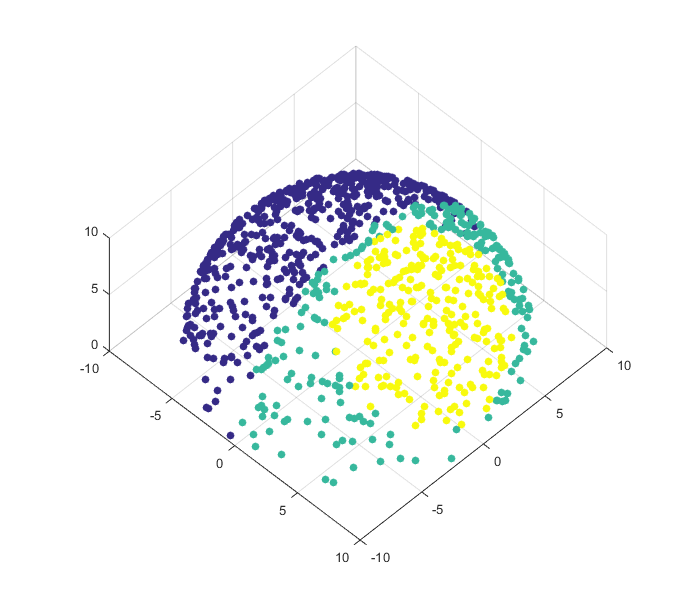
\includegraphics[width=\linewidth]{figures/sphere.png}
            \captionof{figure}{Sphere manifold}
        \end{center}
    \end{minipage}
    %
    \begin{minipage}[b]{0.5\linewidth}
        \begin{center}
            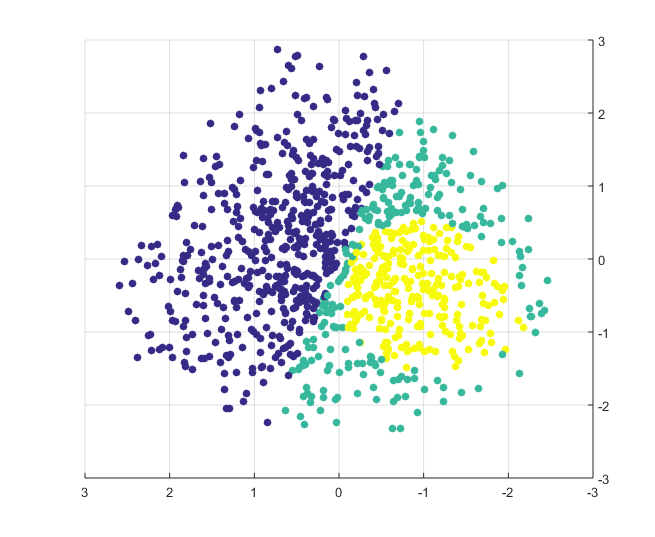
\includegraphics[width=\linewidth]{figures/sphere_result.png}
            \captionof{figure}{Result of Lle algorithm}
        \end{center}
    \end{minipage}

    \subsection*{Result of multidimensional scaling}

    \begin{minipage}[b]{0.5\linewidth}
        \begin{center}
            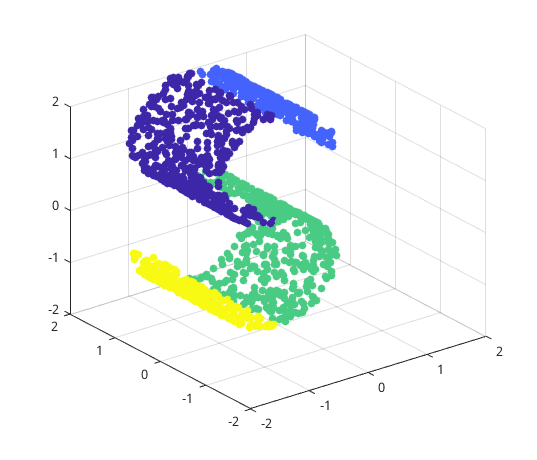
\includegraphics[width=\linewidth]{figures/s_curve.png}
            \captionof{figure}{S curve manifold}
        \end{center}
    \end{minipage}
    %
    \begin{minipage}[b]{0.5\linewidth}
        \begin{center}
            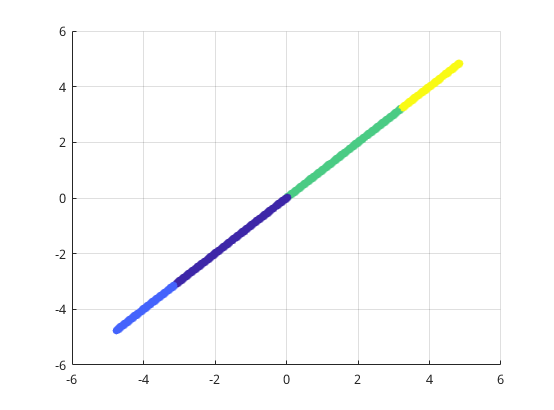
\includegraphics[width=\linewidth]{figures/s_curve_result.png}
            \captionof{figure}{Result of Mds method}
        \end{center}
    \end{minipage}

    \subsection*{Results of both methods with the same manifold}

    \begin{center}
        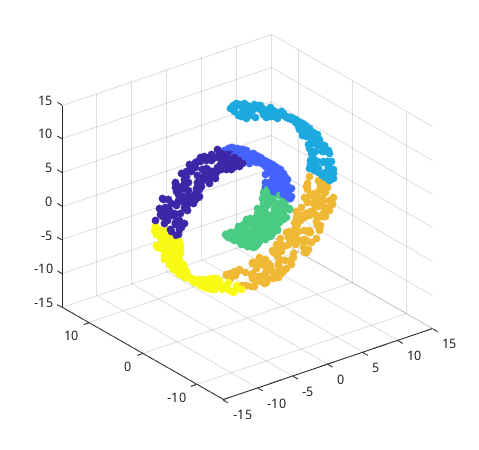
\includegraphics[width=0.5\linewidth]{figures/swiss_roll.png}
        \captionof{figure}{Swiss roll manifold}
    \end{center}

    \begin{minipage}[b]{0.5\linewidth}
        \begin{center}
            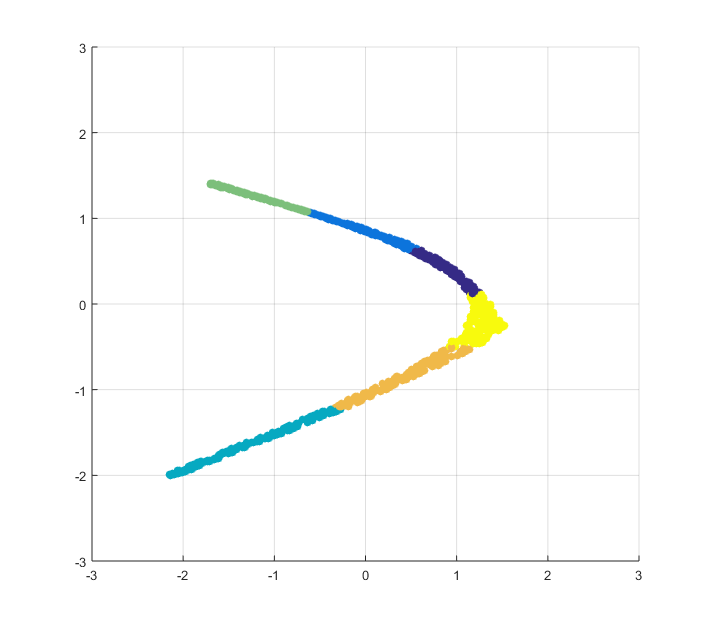
\includegraphics[width=1.0\linewidth]{figures/swiss_roll_result_lle.png}
            \captionof{figure}{Result of Lle algorithm}
        \end{center}
    \end{minipage}
    %
    \begin{minipage}[b]{0.5\linewidth}
        \begin{center}
            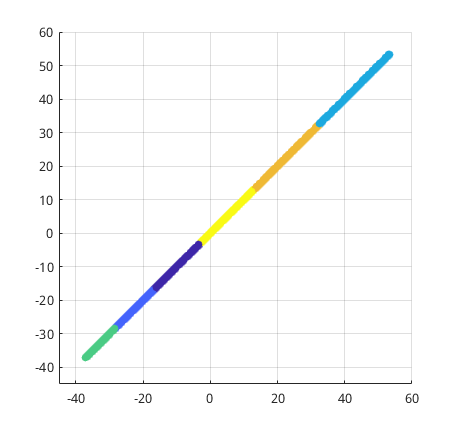
\includegraphics[width=1.0\linewidth]{figures/swiss_roll_result_mds.png}
            \captionof{figure}{Result of Mds method}
        \end{center}
    \end{minipage}

    \section*{Conclusions}

    In this work a theorical and practical develop of the local linear embedding
    algorithm multidimensional scaling method was described. During the process
    it was found that althought the problems started with a quite complicated
    setup, the development of a theorical frameworks  allowed to generate great
    simplifications that reduced the original problems to just solve linear
    systems of equations and eigenvector problems. These simplifications made
    possible the creation of a relatively simple algorithm that can detect low
    dimensional manifolds in multidimensional spaces. This statement is
    supported in the results section where 3 dimensional manifolds were
    simplified to dimension 2 but preserving the intrinsic structure of the
    original dataset.

    \bibliographystyle{unsrt}
    \bibliography{poster}

\end{multicols}
\end{document}
